\documentclass[12pt]{book}
\usepackage[margin=.85in]{geometry} % for MARGIN
\usepackage[many]{tcolorbox}    	% for COLORED BOXES (tikz and xcolor included)


\usepackage{multicol}   
\usepackage{enumerate}
\usepackage[shortlabels]{enumitem}
\usepackage{varwidth}
\usepackage{tasks}
\usepackage[export]{adjustbox}

\usepackage{titleps}
\usepackage{setspace}               % for LINE SPACING
\usepackage[⟨options⟩]{fancyhdr}
\usepackage{enumitem}
\setlist{nosep}
\usepackage{tikz}
\usepackage{pgfplots}
\pgfplotsset{compat=1.5.1}
\usetikzlibrary{datavisualization}
\usetikzlibrary{datavisualization.formats.functions}

\newcommand{\D}{\displaystyle}


\setlength\parindent{0pt}   % killing indentation for all the text
\setstretch{1.3}            % setting line spacing to 1.3
\setlength\columnsep{0.25in} % setting length of column separator
\pagestyle{fancy}           % setting pagestyle to be headings

\usepackage[]{titlesec}

\fancyhead[L]{Math V04 - College Algebra}
\fancyhead[R]{Christina Papazacharioudakis}

\tcbset{
    sharp corners,
    colback = white,
    before skip = 0.2cm,    % add extra space before the box
    after skip = 0.5cm      % add extra space after the box
}                           % setting global options for tcolorbox

    \newtcolorbox{boxR}{
    fontupper = \color{black}, % font color
    boxrule = 1.5pt,
    colframe = black,
    rounded corners,
    arc = 5pt   % corners roundness
}

\definecolor{ballblue}{rgb}{0.13, 0.67, 0.8}

\begin{document}



\begin{comment}
Name: \underline{\hspace{100mm}}
\vspace{20mm}
  \centerline{\Large \textbf{Chapter 2: Equations and Inequalities} } 

{\large
\begin{center}
\begin{varwidth}{\textwidth}
\begin{enumerate}[2.1]
    \item The Regular Coordinate System and Graphs
    \item Linear Equations in One Variable
    \item Models and  Applications (Skipping)
    \item Complex Numbers
    \item Quadratic Equations
    \item Other Types of Equations
    \item Linear Inequalities and Absolute Value Inequalities
\end{enumerate}
\end{varwidth}
\end{center}

}
\newpage  
\end{comment}

\textbf{{\Large 3.1 Functions and Function Notation}}
\vspace{5mm}

We now start a new chapter studying functions! Functions are fundamental in mathematics, as they help us model and analyze real-world situations by describing how one quantity depends on another. Understanding functions will lay the groundwork for exploring more advanced topics in algebra and beyond, so let's get started!
\\

{\large \textbf{Determining Whether a Relation Represents a Function}}
\vspace{3mm}

A \textbf{relation} is a set of ordered pairs. The set of the first components of each ordered pair is called the \textbf{domain} and the set of the second components of each ordered pair is called the \textbf{range}. \\

Consider the following set of ordered pairs. The first numbers in each pair are the first five natural numbers. The second number in each pair is twice that of the first.
$$ \{(1,2), (2,4), (3,6), (4,8), (5,10) \}$$

The domain is: 
\\

The range is: 
\\

The \textbf{input} value or \textbf{independent variable} is often labeled lowercase $x$. Each value in the range is also known as the \textbf{output} value, or \textbf{dependent variable}, often labeled as a lowercase $y$.
\\

A \textbf{function $\mathbf{f}$} is a relation that assigns a single value in the range to each value in the domain. A way you can think about it is that ``each input has exactly one output".  
\\

\centerline{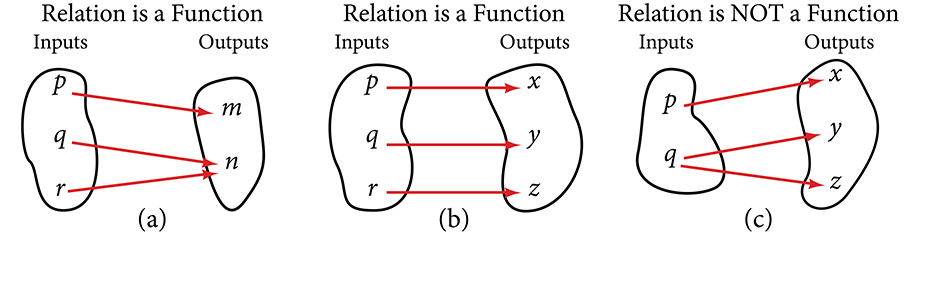
\includegraphics[height=50mm, width=160mm]{Chapter 3/3.1-figure1.jpeg}}

    \newpage
\begin{boxR}
    \textbf{Function}
    \vspace{1mm}
    \hline
    \vspace{2mm}
    A \textbf{function} is a relation in which each possible input value leads to one output value. We say “the output is a function of the input.”

    The \textbf{input} values make up the \textbf{domain}, and the \textbf{output} values form the \textbf{range}.
\end{boxR}

Let's look at some more relations to see if their relationship is a function.

\begin{boxR}
    \textbf{How To}
    \vspace{1mm}
    \hline
    \vspace{2mm}
    \textbf{Given a relationship between two quantities, determine whether the relationship is a function.}
    
    \begin{enumerate}
        \item Identify the input values.
        \item Identify the output values.
        \item If each input value leads to only one output value, classify the relationship as a function. If any input value leads to two or more outputs, do not classify the relationship as a function.
    \end{enumerate}
\end{boxR}
\vspace{3mm}
   \underline{\textbf{Example 1 - Determine If the Menu Price Lists Are Functions}}

    The coffee shop menu, shown below, consists of items and their prices.
    \\
    
    \centerline{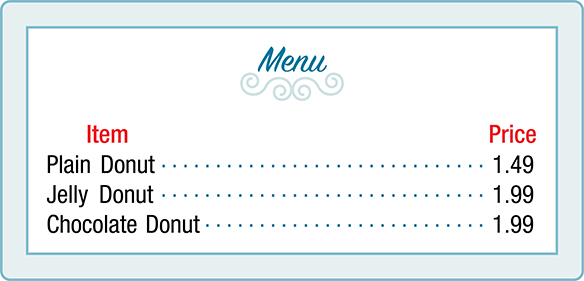
\includegraphics[height=30mm, width=75mm]{Chapter 3/3.1-figure2.jpeg}}
    \begin{multicols}{2}
         \begin{enumerate}[(a)]
        \item Is price a function of the item?
        \vspace{50mm}
        \item Is the item a function of the price?
    \end{enumerate}
    \end{multicols}
   
    
\newpage
{\large \textbf{Using Function Notation}}
\vspace{3mm}

Once we identify that a relation is a function, we want to use function notation to study these relations.
\vspace{3mm}
\begin{boxR}
    \textbf{Function Notation}
    \vspace{1mm}
    \hline
    \vspace{2mm}
    The notation $y=f(x)$ defines a function named $f$. We read this as ``$y$ is a function of $x$". The letter $x$ represents the input value (what we see in parenthesis). $x$ is the independent variable. The letter $y$, or $f(x)$, represents the output value. We call $y$ the independent variable.
    \end{boxR}
\vspace{3mm}
 \underline{\textbf{Example 4 - Interpreting Function Notation}}
 
 A function $N = f(y)$ gives the number of puppies adopted, $N$, in a town per year. What does $f(2005)=900$ represent?


 
\newpage

{\large \textbf{Representing Functions Using Tables}}
\vspace{3mm}

Sometimes we represent a function using a table that displays the correspondence between input and output values. 

As an example, perhaps we look at a function that tells us the number of days in a given month (January = 1, February = 2, and so on). We define a days-in-a-month function $D = f(m)$. The input 
is the month as an integer, and the output is the number of days in a month. 
\vspace{5mm}


\begin{tabular}{ |l|c|c|c|c|c|c|c|c|c|c|c|c| } 
 \hline
 \textbf{Month number, $m$ (input)} & 1 & 2 & 3 & 4 & 5 & 6 & 7 & 8 & 9 & 10 & 11 & 12  \\ 
 \hline
 \textbf{Days in a month, $D$ (output)} & 31 & 28 & 31 & 30 & 31 & 30 & 31 & 31 & 30 & 31 & 30 & 31  \\ 
 \hline
\end{tabular}

\vspace{3mm}
$D(1)=$ \underline{ \hspace{20mm}}

$D(6)=$ \underline{ \hspace{20mm}}

If $D(m)=28$, $m=$ \underline{ \hspace{20mm}}

If $D(m)=30$, $m=$ \underline{ \hspace{30mm}}

\vspace{5mm}
\begin{boxR}
    \textbf{How To}
    \vspace{1mm}
    \hline
    \vspace{2mm}
    \textbf{Given a table of input and output values, determine whether the table represents a function}
    \begin{enumerate}
        \item Identify the input and output values.
        \item Check to see if each input value is paired with only one output value. If so the table represents a function. "For every input, there is exactly one output".
    \end{enumerate}
\end{boxR}

\vspace{1mm}


\underline{\textbf{Example 5 - Identifying Tables that Represent Functions}}

Which tables represent a function (if any)?

\begin{multicols}{3}

\begin{enumerate}
    \item {
        \begin{tabular}{ |c|c| } 
         \hline
         \textbf{Input} & \textbf{Output}  \\ 
           \hline
              $2$ & $1$ \\
             \hline
             $5$ & $3$ \\
             \hline
            $8$ & $6$ \\
         \hline

          \end{tabular} }
    \item {
\begin{tabular}{ |c|c| } 
 \hline
 \textbf{Input} & \textbf{Output}  \\ 
    \hline
    $-3$ & $5$ \\
    \hline
    $0$ & $1$ \\
     \hline
    $4$ & $5$ \\
    \hline
\end{tabular} 
}

\item {
\begin{tabular}{ |c|c| } 
 \hline
 \textbf{Input} & \textbf{Output}  \\ 
    \hline
    $1$ & $0$ \\
    \hline
    $5$ & $2$ \\
     \hline
    $5$ & $4$ \\
    \hline
\end{tabular} 
}
\end{enumerate}
\end{multicols}
\newpage

{\large \textbf{Finding Input and Output Values of a Function}}

\textbf{Evaluation of Functions in Algebraic Forms}

When we know an input value and want to determine the corresponding output value of a function, we \textit{evaluate} the function. Evaluating will always produce one result because each input corresponds to exactly one output.
\\

\begin{boxR}
  \textbf{  Given the formula for a function, evaluate.}
\vspace{1mm}
\hline
\vspace{2mm}
\begin{enumerate}
    \item Substitute the input variable in the formula with the value provided.
    \item Calculate the result.
\end{enumerate}
\end{boxR}

\underline{\textbf{Example 6 - Evaluating Functions at Specific Values}}

Evaluate $f(x)=x^2+3x-4$ at
    \begin{enumerate}[(a)]
    \begin{multicols}{2}
        \item $x=2$
        \item $x=a$
    \end{multicols}
    \vspace{35mm}
    \begin{multicols}{2}
         \item $x=a+h$
     \vspace{30mm}
    \item Find $\D \frac{f(a+h)-f(a)}{h}$
     \vspace{30mm}
    \end{multicols}
   
    \end{enumerate}

\vspace{35mm}



\newpage

\underline{\textbf{Example 7 - Evaluating Functions}}

Given the function $h(p)=p^2+2p$, evaluate $h(4)$.

\vspace{25mm}

When we know an output value and want to determine the input values that would produce that output value, we set the output equal to the function’s formula and solve for the input. Solving can produce more than one solution because different input values can produce the same output value.
\\

\underline{\textbf{Example 8 - Solving Functions}}

Given that $h(p)=p^2 +2p$, solve for $h(p)=3$.

\vspace{70mm}
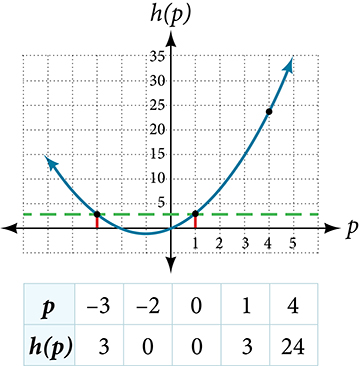
\includegraphics[height=60mm, width=60mm]{Chapter 3/3.1-figure3.jpeg}
\newpage


\underline{\textbf{Example 10 - Expressing the Equation of a Circle as a Function}}

Does the equation $x^2 + y^2 = 1$ represent a function with $x$ as the input and $y$ as the output? Let's see!

\vspace{45mm}

\textbf{Finding Function Values from a Graph}
\\

\underline{\textbf{Example 12 - Reading Function Values from a Graph}}

Given the graph, evalute $f(2)$ and solve $f(x)=4$.
\vspace{5mm}

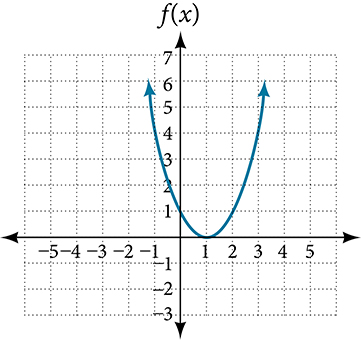
\includegraphics[height=70mm, width=70mm]{Chapter 3/3.1-figure4.jpeg}

\newpage

\textbf{Determining Whether a Function is One-to-One}

Some functions have a given output value that corresponds to two or more input values. We saw this in the previous example, example 12. 

We now look at functions where every output corresponds to one input value. 
\\

\begin{boxR}
   \textbf{ One-to-One Function}
    \vspace{1mm}
    \hline
    \vspace{2mm}
    A \textbf{one-to-one} function is a function in which each output value correspond to one input value.
\end{boxR}

Remember, if we are working with a function, we already have that every input has exactly one output. 
\\

\begin{boxR}
   \textbf{ How To}
   \vspace{1mm}
   \hline
   \vspace{2mm}
   \textbf{Given a relation, determine if it is a one-to-one function.}
   \begin{enumerate}
       \item Determine if the relation is a function: Does every input have exactly one output? If so, go to step 2. If not, the relation is not a function, and therefore cannot be a one-to-one function.
       \item If the relation is a function, determine if it is one-to-one. Does every output come from exactly one input?
   \end{enumerate}
\end{boxR}
\underline{\textbf{Example 13 - Determine Whether a Relation Is a One-to-One Function}}

Determine if the relation represents a one-to-one function of $x$.
\begin{multicols}{3}
    

\begin{enumerate}[(a)]
    \item {
\begin{tabular}{ |c|c| } 
 \hline
 \textbf{$\mathbf{x}$} & $\mathbf{y}$ \\ 
    \hline
    $5$ & $3$ \\
    \hline
    $10$ & $8$ \\
     \hline
    $10$ & $14$ \\
    \hline
\end{tabular} 
}
 \item {
\begin{tabular}{ |c|c| } 
 \hline
 \textbf{$\mathbf{x}$} & $\mathbf{y}$ \\ 
    \hline
    $5$ & $3$ \\
    \hline
    $10$ & $8$ \\
     \hline
    $15$ & $8$ \\
    \hline
\end{tabular} 
}
   \item {
\begin{tabular}{ |c|c| } 
 \hline
 \textbf{$\mathbf{x}$} & $\mathbf{y}$ \\ 
    \hline
    $5$ & $3$ \\
    \hline
    $10$ & $8$ \\
     \hline
    $15$ & $14$ \\
    \hline
\end{tabular} 
}
\end{enumerate}
\end{multicols}


\newpage
\textbf{\large Using the Vertical Line Test}

The \textbf{vertical line test} can be used to determine whether a graph represents a function. If we can draw any vertical line that intersects a graph more than once, then the graph does not define a function because a function has only one output value for each input value.

\vspace{5mm}
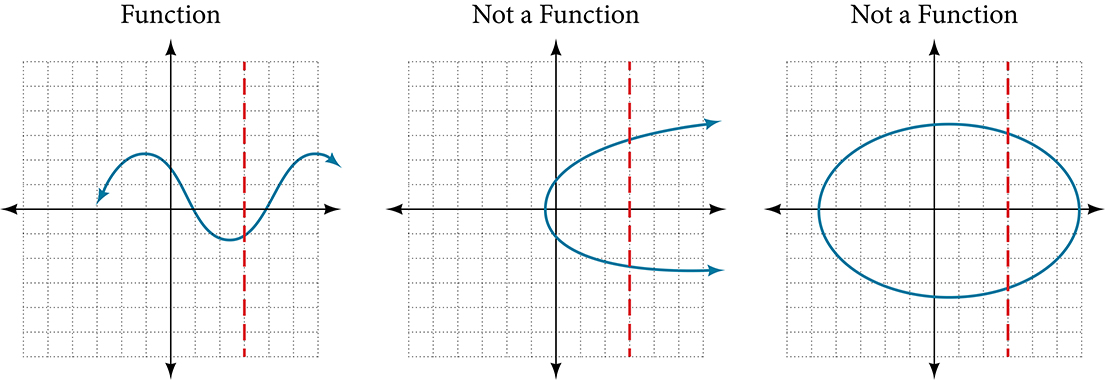
\includegraphics[height=55mm, width=170mm]{Chapter 3/3.1-figure5.jpeg}
\vspace{3mm}
\begin{boxR}
    \textbf{How To}
    \vspace{1mm}
    \hline
    \vspace{2mm}
    \textbf{Given a graph, use the vertical line test to determine if the graph represents a function.}
    \begin{enumerate}
        \item Inspect the graph to see if any vertical line drawn would intersect the curve more than once.
        \item If there is any such line, determine that the graph does not represent a function.
    \end{enumerate}
\end{boxR}

\underline{\textbf{Example 14 - Applying the Vertical Line Test}}
\vspace{3mm}

Which of the graphs represent a function $y=f(x)$?
\\

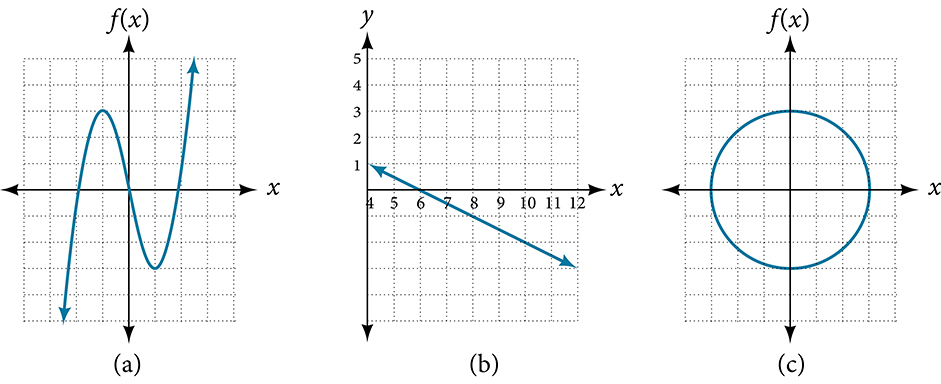
\includegraphics[height=60mm, width=165mm]{Chapter 3/3.1-figure6.jpeg}
\newpage
\textbf{\large Using the Horizontal Line Test}
\\

Once we have determined that a graph defines a function, an easy way to determine if it is a one-to-one function is to use the \textbf{horizontal line test}. Draw horizontal lines through the graph. If any horizontal line intersects the graph more than once, then the graph does not represent a one-to-one function.
\\

\underline{\textbf{Example 15 - Applying the Horizontal Line Test}}
\vspace{3mm}

In the previous example, we found that $(c)$ was not a function. Apply the horizontal line test to $(a)$ and $(b)$ to determine if any of the functions are one-to-one.
\\

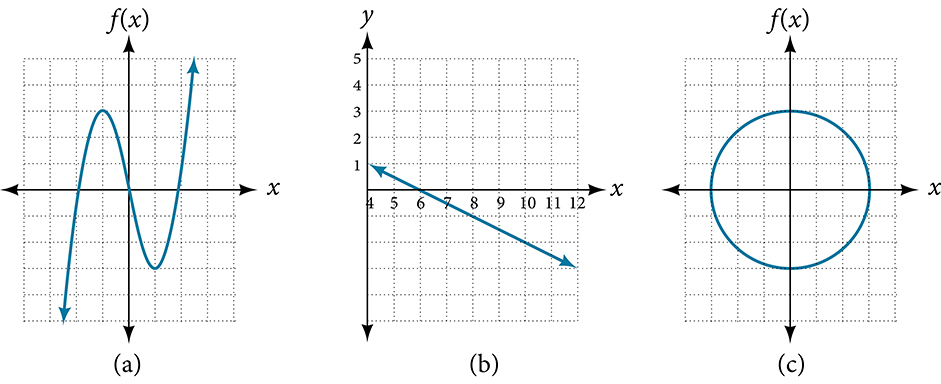
\includegraphics[height=60mm, width=165mm]{Chapter 3/3.1-figure6.jpeg}
\newpage

{\large \textbf{Identifying Basic Toolkit Functions}}

\\

In this chapter, we will be exploring functions—the shapes of their graphs, their unique characteristics, their algebraic formulas, and how to solve problems with them. 

%When learning to read, we start with the alphabet. When learning to do arithmetic, we start with numbers. When working with functions, it is similarly helpful to have a base set of building-block elements. We call these our “toolkit functions,” which form a set of basic named functions for which we know the graph, formula, and special properties.
%\\

\textbf{Toolkit Functions}
\\

 \begin{tabular}{ |c|c|c| } 
         \hline
              \textbf{Name} & \textbf{Function} & \textbf{Graph} \\
             \hline
             Constant & $f(x)=c$ where $c$ is a constant & 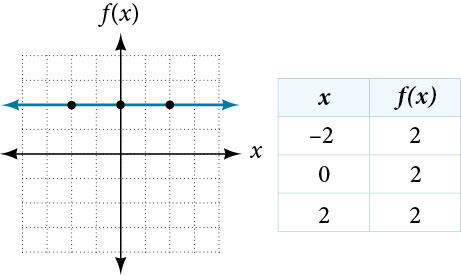
\includegraphics[]{Chapter 3/3.1-figure7.jpeg} \\
             \hline
            Identity & $f(x)=x$ & 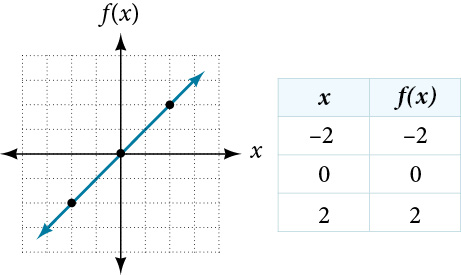
\includegraphics[]{Chapter 3/3.1-figure9.jpeg}\\
            \hline
            Absolute Value & $f(x)=|x|$ & 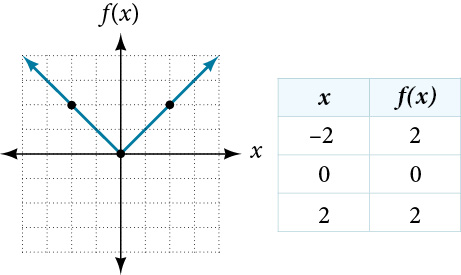
\includegraphics[]{Chapter 3/3.1-figure10.jpeg} \\
            \hline
             Quadratic & $f(x)=x^2$ & 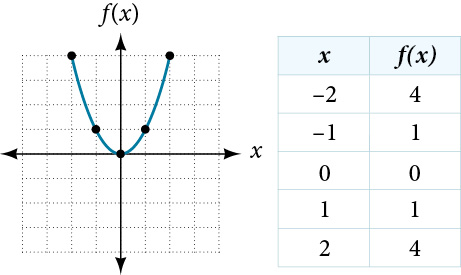
\includegraphics[]{Chapter 3/3.1-figure11.jpeg}\\
            \hline
          \end{tabular} 

\newpage

 \begin{tabular}{ |c|c|c|} 
         \hline
              \textbf{Name} & \textbf{Function} & \textbf{Graph} \\
            \hline
            Cubic & $f(x)=x^3$  &  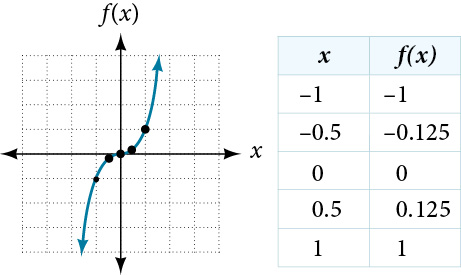
\includegraphics[scale=1]{Chapter 3/3.1-figure12.jpeg}\\
            \hline
            Reciprocal & $f(x) = \frac{1}{x}$ &  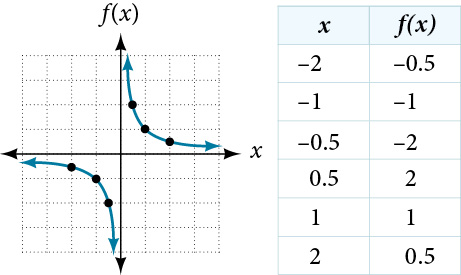
\includegraphics[]{Chapter 3/3.1-figure13.jpeg} \\
            \hline
            Reciprocal Squared & $f(x)=\frac{1}{x^2}$ & 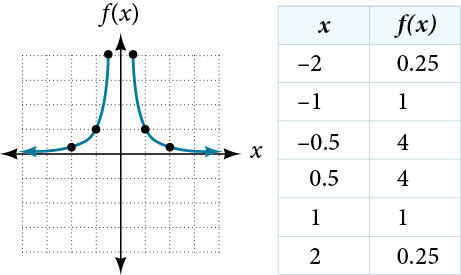
\includegraphics[]{Chapter 3/3.1-figure14.jpeg}\\
            \hline
            Square Root & $f(x)=\sqrt{x}$ & 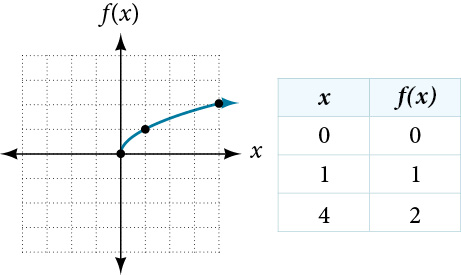
\includegraphics[]{Chapter 3/3.1-figure15.jpeg}\\
            \hline
            Cube Root & $f(x)=\sqrt[3]{x}$ & 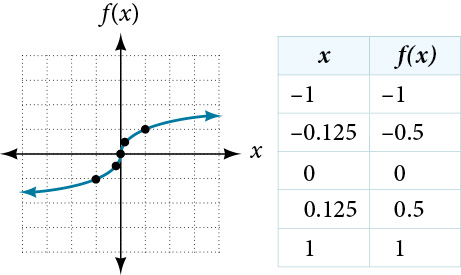
\includegraphics[]{Chapter 3/3.1-figure16.jpeg}\\
            \hline
             \end{tabular}










\end{document}


